\section{Durchführung und Aufbau}
\label{sec:Durchführung}

\subsection{Zeitabhängigkeit der Schwingungsamplitude}
In der Abbildung \ref{fig:Durch1} ist eine Schaltung aufgebaut, mit welcher die Zeitabhängigkeit der Schwingungsamplitude untersucht werden kann. Um die Abklingdauer $T_\text{ex}$ und den effektiven Dämpfungswiderstand $R_\text{eff}$ zu bestimmen, wird die Amplitudenabnahme eines gedämpften RCL-Schwingkreises untersucht.

\begin{figure}
  \centering
  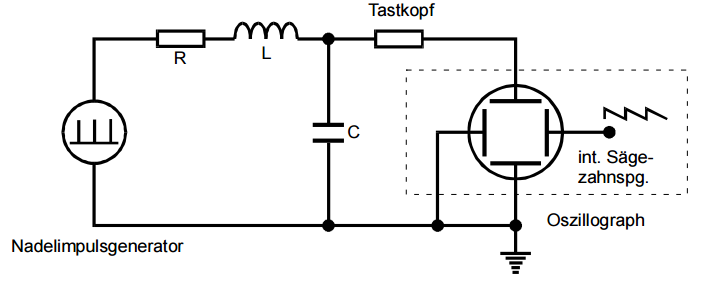
\includegraphics[height=4cm]{picture/Durch1.PNG}
  \caption{Aufbau eines RCL-Schwingkreises zur Untersuchung der Spannung am Kondensator \cite[294]{sample}.}
  \label{fig:Durch1}
\end{figure}

Der Nadelimpulsgenerator wird so eingestellt, dass die Spannungsamplitude $U_\text{C}$, welche am Kondensator abgenommen wird, um den Faktor 3 bis 8 kleiner wird. Die Spannung wird am Oszilloskop gegen die Zeit aufgetragen, die Werte werden auf einem USB-Stick gespeichert und mit Hilfe von Python 3.4.3 ausgewertet.

\subsection{Bestimmung des aperiodischen Grenzwiderstandes}
In der Abbildung \ref{fig:Durch2} ist eine Schaltung aufgebaut, mit welcher der aperiodische Grenzwiderstand $R_\text{ap}$ bestimmt werden kann.

\begin{figure}
  \centering
  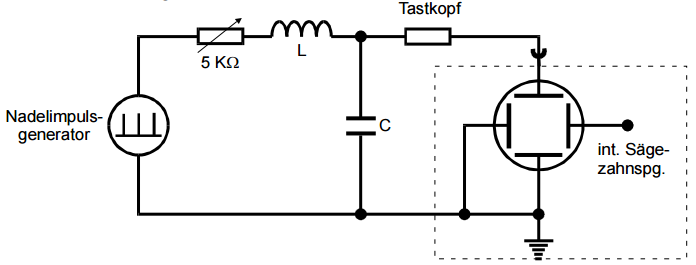
\includegraphics[height=4cm]{picture/Durch2.PNG}
  \caption{Aufbau eines RCL-Schwingkreises zur Bestimmung des aperiodischen Grenzwiderstandes \cite[295]{sample}.}
  \label{fig:Durch2}
\end{figure}

Der regelbare Widerstand wird auf seinen maximal Wert eingestellt, so dass der Schwingkreis ein reines Relaxationsverhalten, also eine monoton abfallende Spannung, zeigt. Nun wird der regelbare Widerstand solange verringert, bis ein Überschwingen der Spannung zu sehen ist. Allerdings ist der Schwingfall dann bereits eingetreten und der Widerstand muss nun solange erhöht werden, bis dieses Phänomen gerade wieder verschwindet. Der nun eingestellte Widerstand wird als $R_\text{ap}$ notiert.

\subsection{Frequenzabhängigkeit der Kondensatorspannung und der Phasenverschiebung}
In der Abbildung \ref{fig:Durch3} ist eine Schaltung aufgebaut, mit welcher die Frequenzabhängigkeit der Kondensatorspannung und der Phasenverschiebung(zwischen Erreger- und Kondensatorspannung) untersucht wird.

\begin{figure}
  \centering
  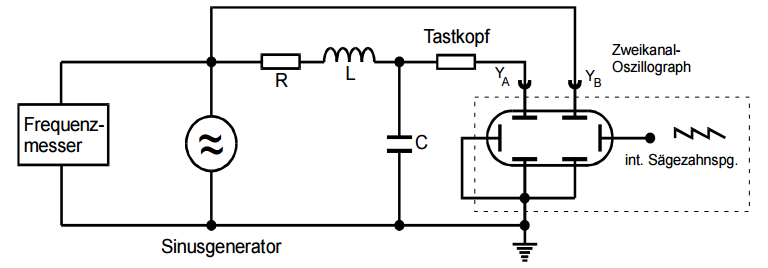
\includegraphics[height=4cm]{picture/Durch3.PNG}
  \caption{Schaltung zur Messung der Frequenzabhängigkeit von der Kondensatorspannung und der Phasenverschiebung \cite[296]{sample}.}
  \label{fig:Durch3}
\end{figure}

Auf dem Oszilloskop wird nun, wie in Abbildung \ref{fig:Durch4} schematisch dargestellt, die Erreger- und die Kondensatorspannung gegen die Zeit aufgetragen. Daraufhin wird die Frequenz $\nu$ am Sinusgenerator im Berreich von (1 - 100000)Hz variiert. Dabei werden etwa 30 Wertepaare aus der Spannung $U_\text{C}$, der Frequenz $\nu$ und der Phasenverschiebung $\Phi$ notiert. Der Bereich um die Resonanzfrequenz wird in kleineren Schritten gemessen, weil diese in der Auswertung genauer betrachtet werden soll. Für die Phasenverschiebung $\Phi$ wird der zeitliche Unterschied der Null durchgänge $a$ gemessen und die Periodenlänge $b$ aus der Frequenz $\nu$ berechnet.   

\begin{figure}
  \centering
  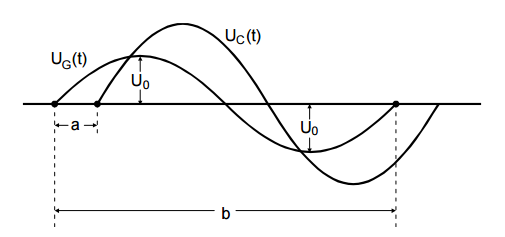
\includegraphics[height=4cm]{picture/Durch4.PNG}
  \caption{Schematische Darstellunf des am Oszilloskop zu sehenden Bildes \cite[282]{samples}.}
  \label{fig:Durch4}
\end{figure}
